\section{Experiment Setup}

\subsection{Product Data Source and Extraction}

The product catalogue is constructed from the source PDF \emph{Great Whiskeys}. We first use PyMuPDF to extract page-level text, embedded images, and page renderings. The extracted text is then parsed into product-level records using a rule-based parser tailored to the layout of this catalogue. Each record corresponds to one whisky expression rather than one PDF page. The final parsed catalogue contains 533 product records from 360 source pages.

Each product record contains structured metadata and descriptive fields, including product name, brand or distillery, style, region, country, age, ABV, product tasting notes, and shared brand or distillery context. Product images are obtained from the extracted catalogue images. Since the raw extracted images often contain large blank regions or page-level artifacts, we apply an image-cropping step that removes surrounding whitespace and keeps the main bottle region. The resulting cropped image is used as the product-side visual evidence.

Here is a sample production of the structured product text and cropped product image for one catalogue entry:
\begin{displayquote}
\textbf{title:} ARDBEG 10-YEAR-OLD | \textbf{text:} Name: ARDBEG 10-YEAR-OLD

\textbf{Brand:} ARDBEG

\textbf{Style:} Single Malt

\textbf{Region:} Islay

\textbf{Country:} Scotland

\textbf{Age:} 10

\textbf{ABV:} 46

\textbf{Product notes:} This non chill-filtered malt has notes of creosote, tar, and smoked fish on the nose. Any sweetness on the tongue quickly dries to a smoky finish.

\textbf{Brand context:} If Islay is the spiritual home of Scotland's pungent, peatsmoked whiskies, then Ardbeg is undoubtedly one of the island's leading disciples. The distillery was first licensed in 1815 in the parish of Kildalton, on Islay's southern coast just beyond Lagavulin and Laphroaig. Reliance on the blending market left Ardbeg in a vulnerable position, however, and when “the whisky loch” became full to the brim in the early 1980s, the distillery was mothballed. In 1997, Ardbeg was rescued by Glenmorangie, who paid a reported £7m and then spent a further £1.4m on upgrading the distillery. At first, the years of non-production caused problems but, as the gaps in the inventory receded, the distillery was finally able to release a standard 10-yearold bottling. Since then, there has been a raft of new bottlings, which have added to Ardbeg's growing cult status among fans of Islay's smoky malt whiskies.

\end{displayquote}

\begin{figure}[h]
    \centering
    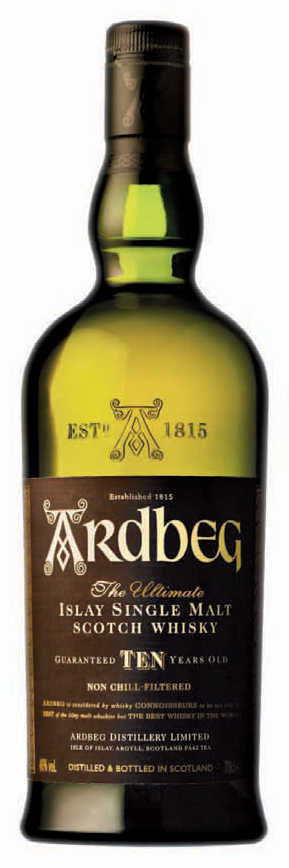
\includegraphics[width=0.15\textwidth]{assets/embedded_image_01.crop.png}
    \caption{The cropped product image for the Ardbeg 10-Year-Old entry, which is used as the visual evidence for embedding construction.}
    \label{fig:my_figure}
\end{figure}

\subsection{Query Set Construction}

We construct three query sets corresponding to the three query modalities. The text query set contains 20 natural language queries. These queries are designed to cover four cases: direct brand lookup, semantic brand-description lookup, ABV-oriented lookup, and flavour-oriented lookup. The relevant product identifiers for these queries are generated from catalogue metadata and tasting descriptions using rule-based keyword and field matching, followed by manual inspection for obvious issues.

The image query set is based on 11 movie or television scene references that contain recognizable whisky bottles. For each reference, we keep two query images. The first is a manually cropped bottle image from the scene, and the second is the whole scene image. This produces 22 image-only queries: 11 cropped-bottle queries and 11 whole-scene queries. The purpose of this split is to measure how much retrieval quality changes when the query image is clean and product-centric versus noisy and contextual.

The image-text query set uses the same 11 whole scene images. Each query pairs the whole scene image with the textual question ``What is the whisky in this image?'' This setting is intended to test native multimodal retrieval, where the query includes both visual evidence and an explicit textual intent.

Representative examples of the query sets are shown below.

\begin{center}
\begin{tabular}{p{0.28\textwidth}p{0.06\textwidth}p{0.58\textwidth}}
\hline
\textbf{Query type} & \textbf{Q/A} & \textbf{Statement} \\
\hline
Direct brand text & Q & I want an Ardbeg whisky. \\
\cline{2-3}
 & A & The four parsed Ardbeg expressions in the catalogue. \\
\hline
Semantic brand text & Q & I want whisky from the southern coast of Islay, famous for pungent heavily peated malts. \\
\cline{2-3}
 & A & The same four Ardbeg products, labelled from the shared brand description without naming Ardbeg in the query. \\
\hline
ABV text & Q & I want Laphroaig cask strength whisky around 57 percent ABV. \\
\cline{2-3}
 & A & The parsed Laphroaig 10-Year-Old Cask Strength product. \\
\hline
Flavour text & Q & I want smoky peaty whisky with seaweed iodine tar and a long coastal finish. \\
\cline{2-3}
 & A & Products whose tasting notes contain related smoky, peaty, coastal, tar, seaweed, iodine, or long-finish descriptors. \\
\hline
\end{tabular}
\end{center}

\begin{center}
\begin{tabular}{p{0.28\textwidth}p{0.06\textwidth}p{0.58\textwidth}}
\hline
\textbf{Query type} & \textbf{Q/A} & \textbf{Statement} \\
\hline
Cropped image & Q & 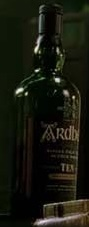
\includegraphics[width=0.1\textwidth]{assets/query_example_ardbeg_crop.jpg} \\
\cline{2-3}
 & A & The four parsed Ardbeg expressions in the catalogue. \\
\hline
Whole-scene image & Q & 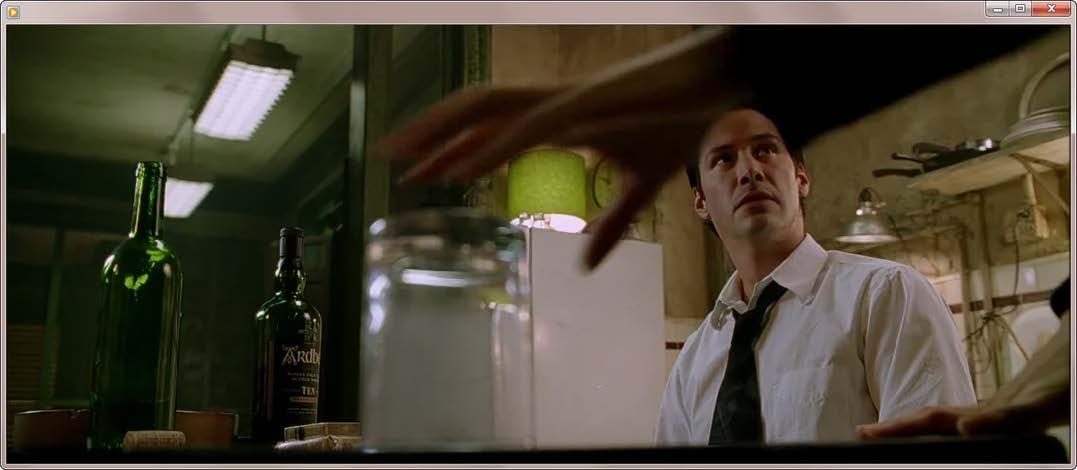
\includegraphics[width=0.30\textwidth]{assets/query_example_ardbeg_scene.jpg} \\
\cline{2-3}
 & A & The four parsed Ardbeg expressions in the catalogue. \\
\hline
Image + text & Q & 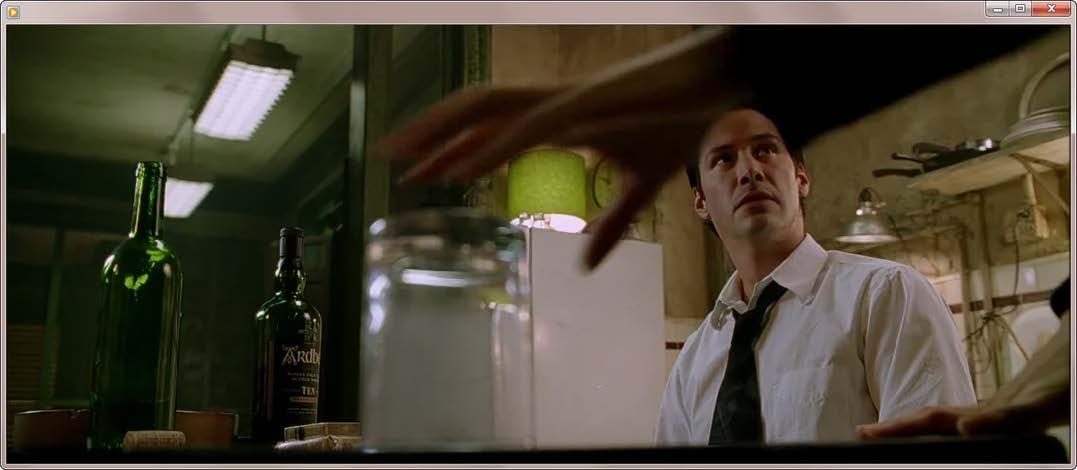
\includegraphics[width=0.30\textwidth]{assets/query_example_ardbeg_scene.jpg} 

Text: ``What is the whisky in this image?'' \\
\cline{2-3}
 & A & The four parsed Ardbeg expressions in the catalogue. \\
\hline
\end{tabular}
\end{center}

\begin{figure}[h]
    \centering
    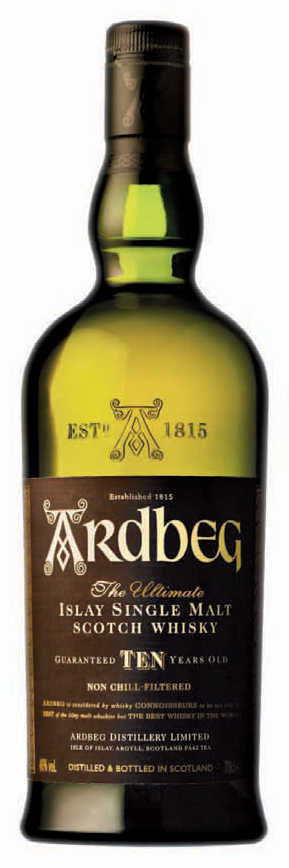
\includegraphics[width=0.1\textwidth]{assets/expected_product_ardbeg_10_crop.png}
    \caption{Representative expected product for the visual Ardbeg queries: Ardbeg 10-Year-Old. The full relevance set contains four parsed Ardbeg expressions.}
    \label{fig:visual_query_expected_product}
\end{figure}

\subsection{Embedding Construction}

All real embeddings are generated with Gemini Embedding 2 using 768-dimensional output vectors. For each product, we build three embedding representations:
\begin{enumerate}
    \item product text embedding, using the structured product text only;
    \item product image embedding, using the cropped catalogue bottle image only;
    \item product multimodal embedding, using both the structured product text and the cropped catalogue bottle image.
\end{enumerate}

The structured product text is built by concatenating the available metadata and description fields into a labelled document. This includes the product name, brand, style, region, country, age, ABV, product notes, and brand context. For multimodal product embeddings, this structured text is paired with the cropped product image.

Queries are embedded according to their modality. Text queries are embedded as text. Image-only queries are embedded from their query image, which may be either a cropped scene bottle or a whole scene image. Image-text queries are embedded by pairing the whole scene image with the question ``What is the whisky in this image?''

\subsection{Embedding Inventory}

The resulting embedding inventory is summarized as follows:

\begin{center}
\begin{tabular}{lll}
\hline
\textbf{Embedding group} & \textbf{Input embedded} & \textbf{Count} \\
\hline
Product text & Structured product text & 533 \\
Product image & Cropped catalogue bottle image & 533 \\
Product multimodal & Structured product text + cropped bottle image & 533 \\
Text queries & Natural language text queries & 20 \\
Image queries & 11 cropped bottle images + 11 whole scene images & 22 \\
Image-text queries & Whole scene image + textual question & 11 \\
\hline
\end{tabular}
\end{center}

These vectors support both the primary modality-matched retrieval settings and the cross-representation ablations. In the primary settings, text queries are matched to product text embeddings, image queries are matched to product image embeddings, and image-text queries are matched to product multimodal embeddings. In the ablations, text and image queries are also matched against the product multimodal embeddings to test whether richer product-side representations improve single-modality search.
